\documentclass{article}
\usepackage[utf8]{inputenc}


\usepackage{graphicx} % Allows including images
\usepackage{subcaption}

\title{Weekly Report 726}
\author{Junior Team }
\date{July 2020}

\begin{document}

\maketitle

\section{Introduction}
This week we had a smaller group than usual as Natalie and Joah had family obligations. We continued to look into the square data set as well as begin to examine their corresponding simulated trajectories. 

\section{Improving then Square Data Set}
\subsection{Pre-Impact Velocity}
Since the objects velocities are derived from position measurements, noise in the position can lead to extremely inaccurate velocity measurements which are amplified by the time step ($v_1 = \frac{x_0 + x_1}{dt}$).
To combat that, often a filter is applied to the data to smooth our the noise, The issue with the filter however, is it also tends to smooth out instantaneous events (like impacts). To combat this, we decided to use a linear fit to a range of positions before and after the impact. We then took the slope of those two lines as the pre and post impact velocities. Theoretically also checks out because the only external force acting on the object is gravity meaning $\dot{x}$ and $\dot{\theta}$ should be constant while $\dot{y}$ is decreasing lineally.\\

\noindent As you can see in the figure below (Fig. \ref{fig:xt6}, Fig. \ref{fig:yt6}) sometimes the filter will lead to a intermediary velocity which is inaccurate. This method also works to simply reduce the effect of any inaccurate measurements. by taking the mean. 


\begin{figure}[h!]
    \centering
     \begin{subfigure}[b]{0.45\linewidth}
            \centering
            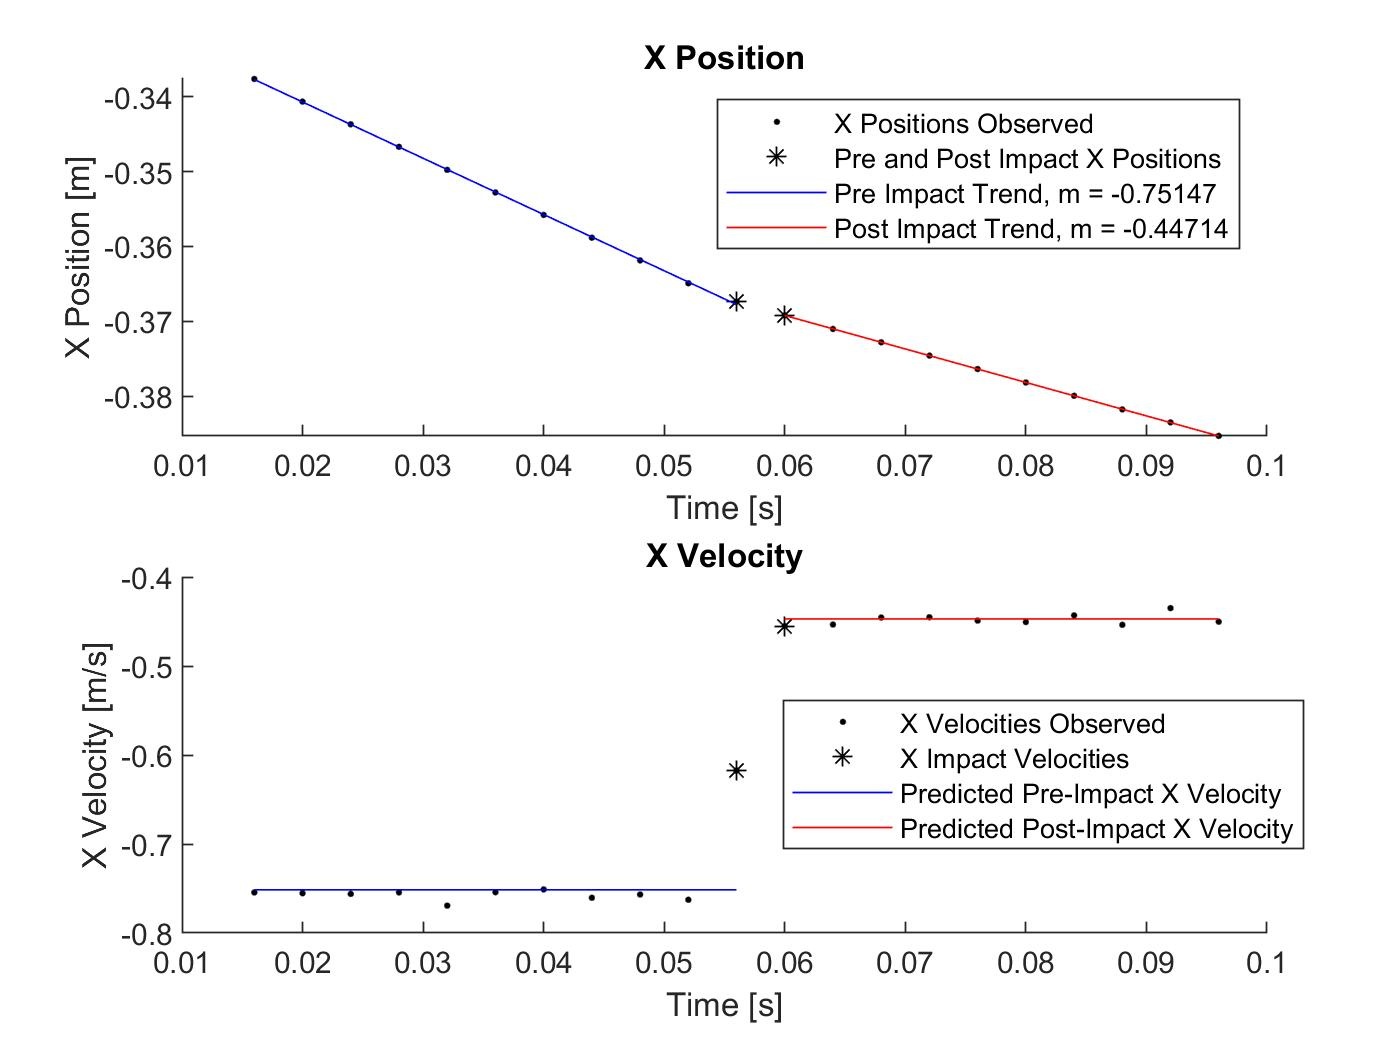
\includegraphics[scale=0.125]{xTrial6.jpg}
            \caption{X Position and Velocity}
            \label{fig:xt6}
    \end{subfigure}
    \quad
    \begin{subfigure}[b]{0.45\linewidth}
            \centering
            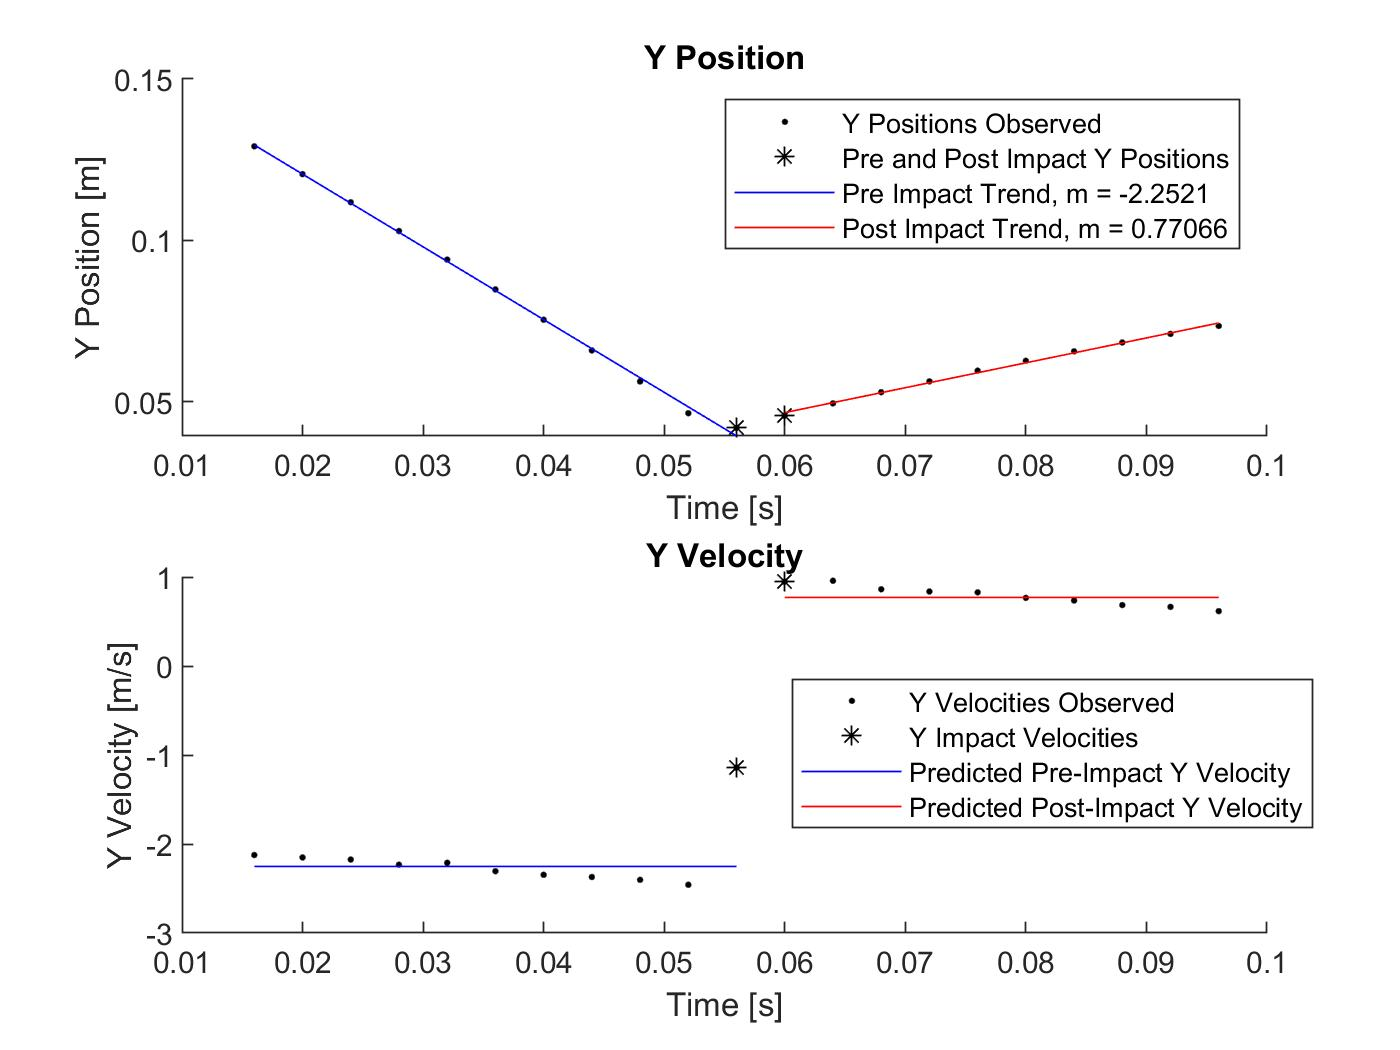
\includegraphics[scale=0.125]{yTrial6.jpg}
            \caption{Y Position and Velocity}
            \label{fig:yt6}
    \end{subfigure}
    \caption{Fitting Position Curves to Find Velocity for Trial 6}
\end{figure}


\subsection{Outliers}
The next step towards improving the square data set was to re-run all of the outliers  on the error graph through our data visualizer to reinspect the cases. There were some double bounces which we had misses or accidentally mislabeled and there were some cases where although it wasn't a double impact, two impacts occurred in quick succession. This would create issues when using the method described in the section above, since it requires points both before and after the impact when doing a linear fit. These cases were also discarded. In addition, Dr. Posa suggested we discard cases where the initial rotational velocity was extremely high (over 50 rad/s), 

\subsection{Improvement in Results}
Next, we took our data set and re-ran it through the IRB model to see how it compared to the original data set we had come up with. The mean for the original square data set was around 0.21 which is a significant decrease for the new data set (over 50\%). 

 \begin{figure}[h!]
        \centering
        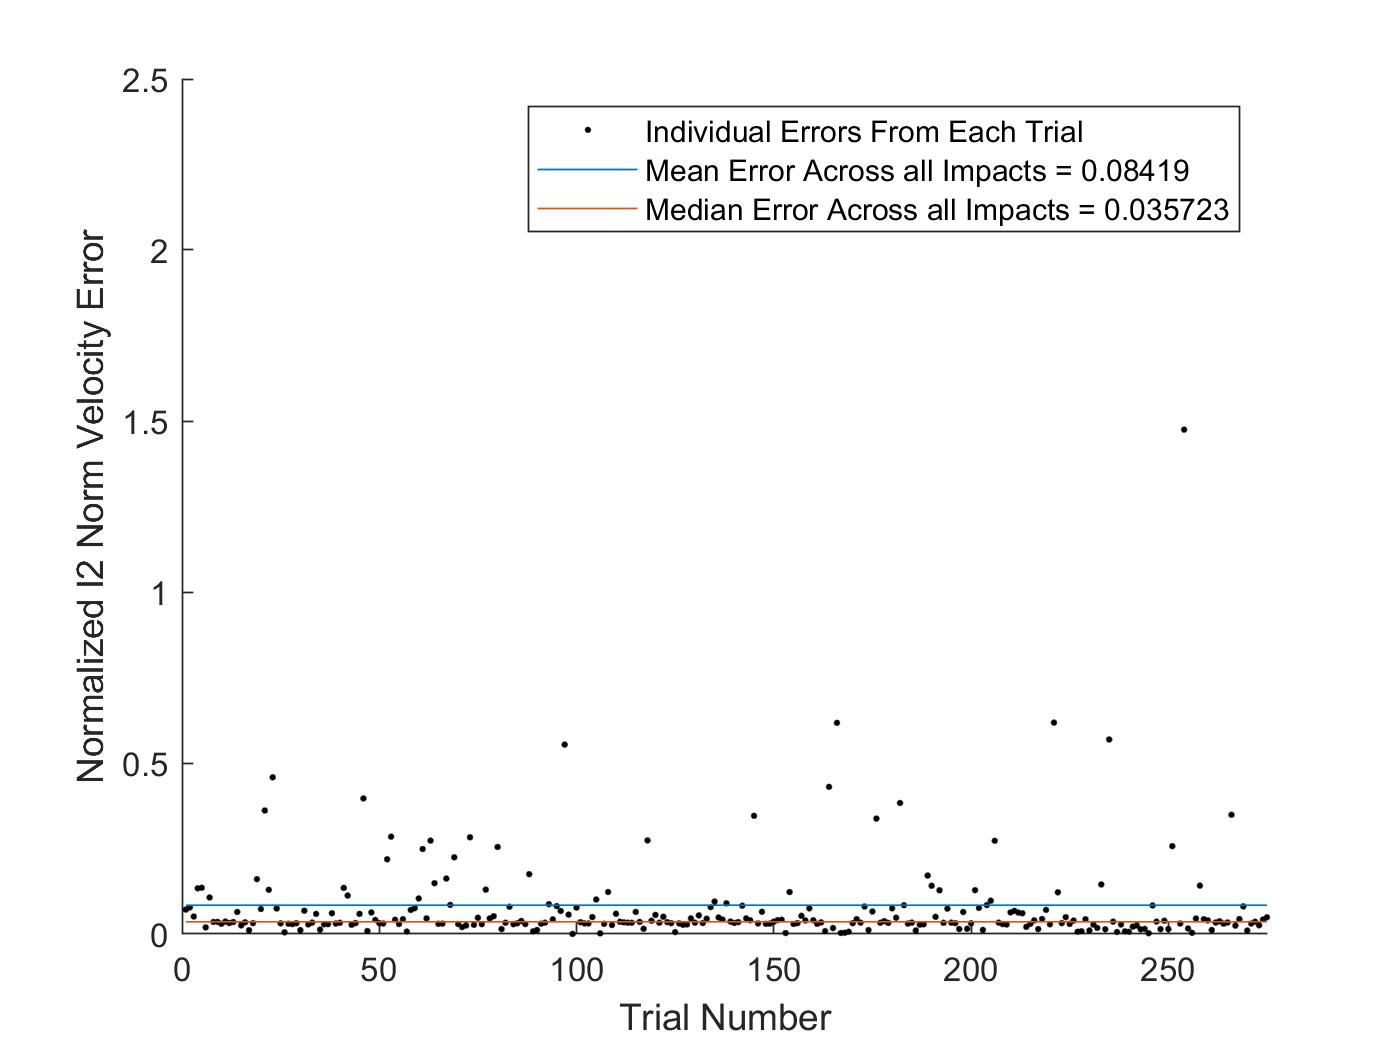
\includegraphics[scale=0.15]{IRBError.jpg}
        \caption{Error Plot for Classical IRB with Updated Square Data Set}
        \label{fig:IRBError}
\end{figure}


\section{Simulated Trajectories}


\subsection{Visualizer}
We adapted our visualizer to show both the actual and simulated trajectories simultaneously in subplots. To our surprise, the simulated trajectories were quite different from the observed trajectories. Often times, the deviations began before any impact even occurred. This led us to wonder how Dr. Fazeli had simulated them in the first place. Will helped us learn that they were simulated using pybullet.

 \begin{figure}[h!]
        \centering
        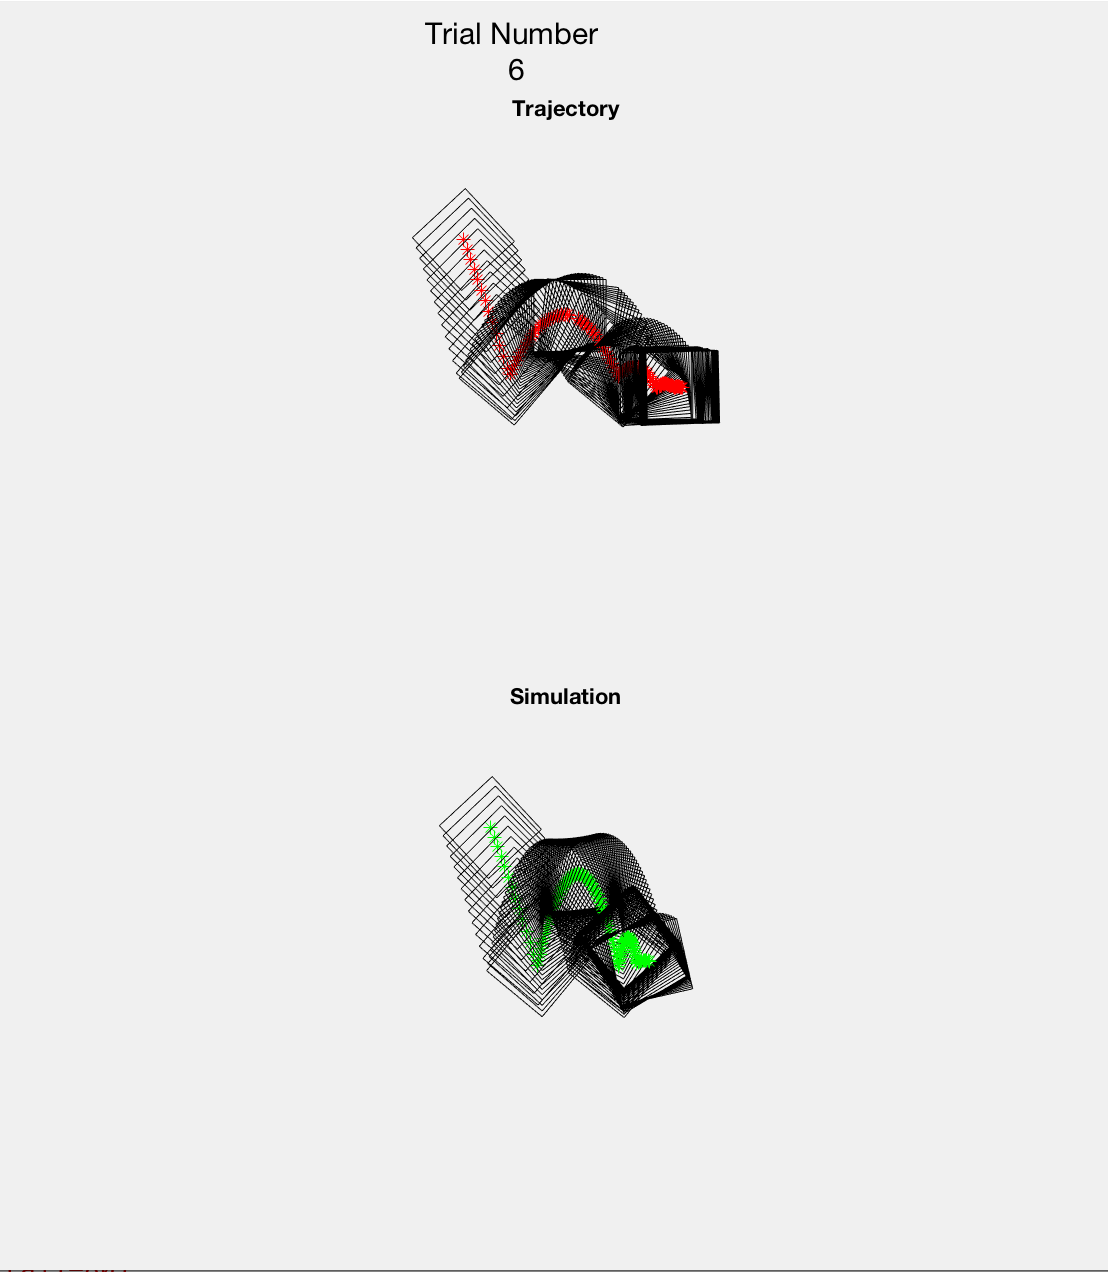
\includegraphics[scale=0.5]{Captura de pantalla 2020-08-03 a la(s) 13.51.25.png}
        \caption{Live comparison of the Real vs Simulated Trajectory}
        \label{fig:RealvsSim}
\end{figure}

\subsection{Comparing the Real vs Simulated Errors}
After going through the simulated data in a similar way we had done with the real data, we manually selected the impacts that we thought were acceptable. In the vast majority of the cases, we found that the cases that we considered "good" in the real data set did not directly coincide with those that we considered "good" in the simulated data set. Anyways, we took 260 cases from each group, and made the following plot that can be seen below. In essence, we discovered that on average, the simulated data gives a lower velocity error, which is four times lower than the real data set. This difference is still the case even when we remove the outliers from the real data set.

\begin{figure}[h!]
        \centering
        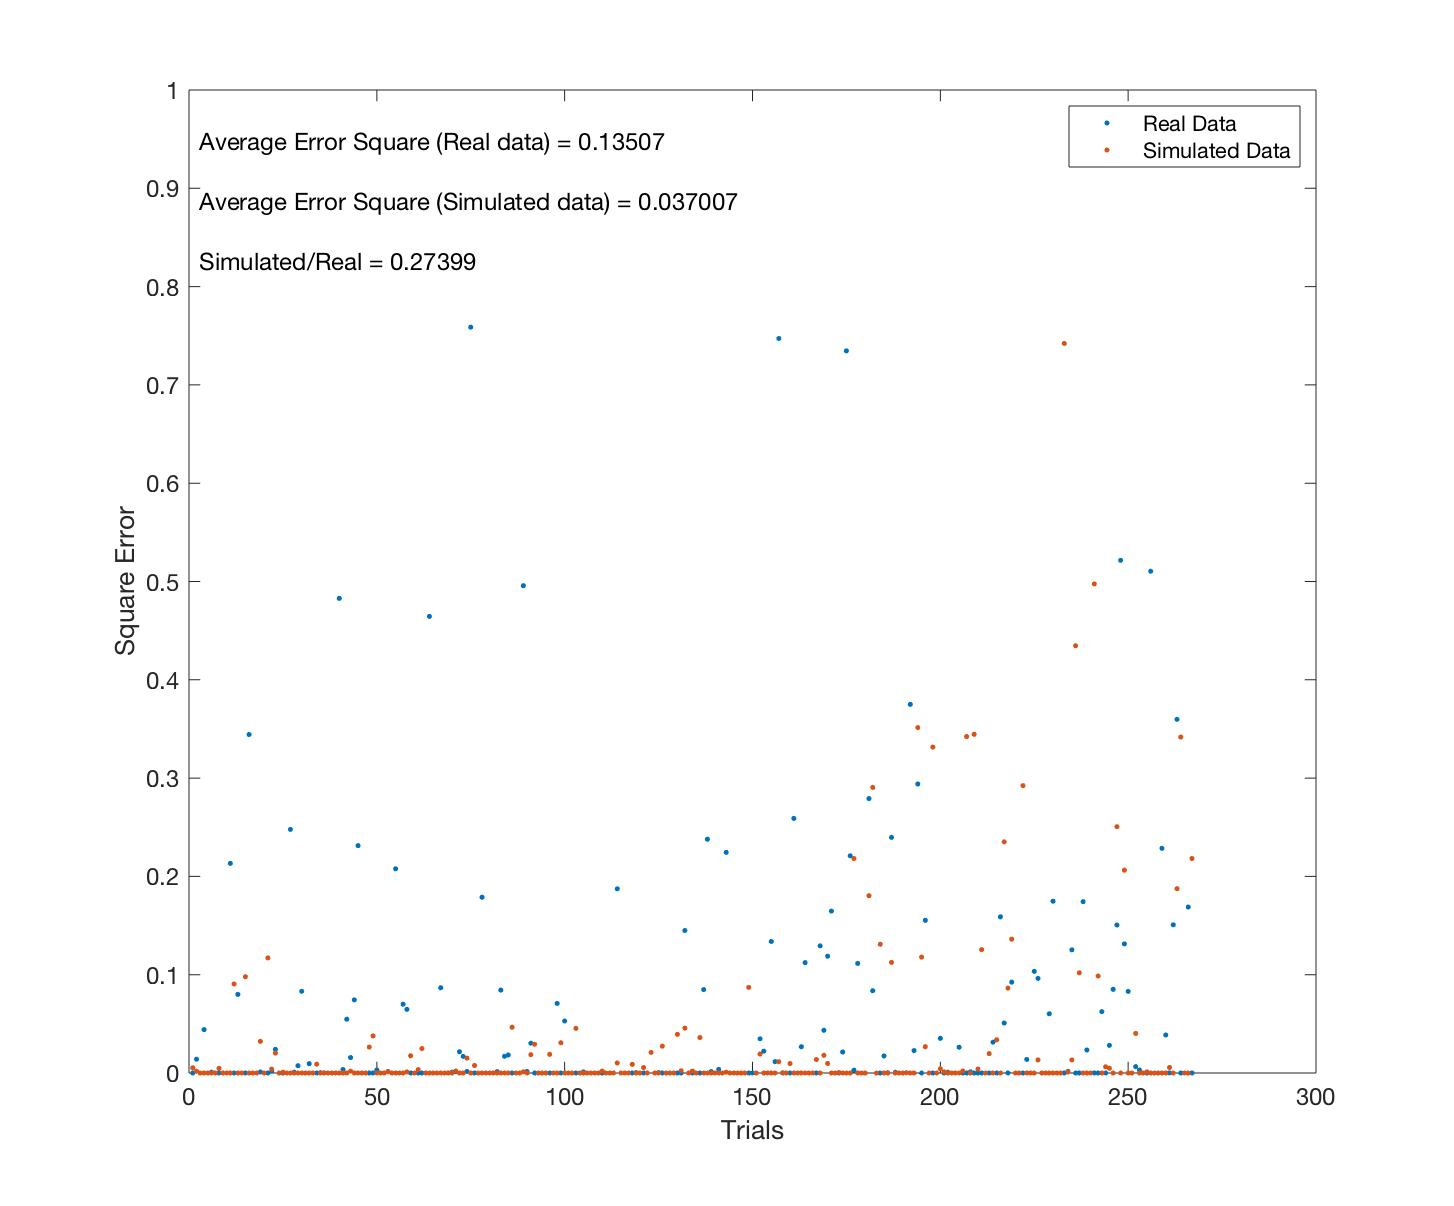
\includegraphics[scale=0.15]{Simulated vs Real.jpg}
        \caption{Error comparison of the Real vs Simulated Trajectory}
        \label{fig:RealvsSimError}
\end{figure}

\end{document}
